\documentclass[fontsize=12pt]{scrartcl}
\usepackage[ngerman]{babel}
\usepackage[utf8]{inputenc}
%\usepackage[latin1]{inputenc}
\usepackage{amsmath}
\usepackage{amstext}
\usepackage{amssymb}
\usepackage{stmaryrd}
\usepackage{verbatim}
\usepackage{mathrsfs}
\usepackage{extarrows}
\usepackage[arrow, matrix, curve]{xy}
\usepackage[centering,includeheadfoot,margin=2cm]{geometry}
\usepackage{gensymb}
\usepackage{graphicx}
\usepackage{framed}
\usepackage{xcolor}
\usepackage{float}
\usepackage{extarrows}
\usepackage{graphicx} 
\usepackage{sidecap}
\usepackage{blindtext,wrapfig}
\usepackage{epstopdf}
\usepackage{import}
\usepackage{fancyhdr}
\usepackage{fancybox}
\usepackage{graphicx}
\usepackage{caption}
\usepackage{subcaption}
\DeclareGraphicsRule{.tif}{png}{.png}{`convert #1 `basename #1 .tif`.png} 
\newcommand{\define}{\ensuremath{\mathrel{\mathop:}=}} % hübscheres :=, da = zentriert wird relativ zu :
\renewcommand{\l}{\left\vert}
\renewcommand{\r}{\right\vert}
\pagestyle{fancy}
\fancyhf{}
\fancyhead[R]{Physikalisches Praktikum 1}
\fancyhead[L]{Marcel Wuttke, Gentian Rrafshi}
\fancyfoot[R]{\thepage}
\fancyfoot[L]{\today}

\begin{document}

\begin{minipage}{\textwidth}
\begin{center}\large
\title{E45e Wirbelstrombremse
 \\
		~\\
		~\\
		Assistent: \\
		 Ralf Albrecht \\
		 ~\\
		Datum Versuchsdurchführung: \\
		22.05.2015}

\author{bearbeitet von\\
~\\
		Gruppe E-041: \\
		Marcel Wuttke Matrnr. 2786678 \\
		Gruppe 3-031: \\
		Gentian Rrafshi Matrnr. 2721617 }
		
\date{\today}

\maketitle

\end{center}
\end{minipage}

\newpage

\tableofcontents

\newpage
\noindent

\section{ Versuchsziel}

Es wird die Bremskraft einer Wirbelstrombremse in Abhängigkeit zum Scheibenmaterial, dem Magnetfeld, der Feldgeometrie und dem Radius betrachtet und ausgewertet.

\section{ Grundlagen}

Wirbelströme sind die Grundlage dieses Versuchs. Ist Induktion im Spiel, so entstehen in Leiterschleifen Flussänderungen. Diese erzeugen Spannungen und Kreisströme, welche wiederum Magnetfelder erzeugen. Die Magnetfelder wirken nach der Lenzschen Regel entgegen der Bewegungsrichtung der Flussänderung. Diese Kreisströme werden dann Wirbelströme genannt. Sie sind oft nicht gewollt, jedoch findet sie eine Anwendung bei den sogenannten Wirbelstrombremsen. Dort wird die Kraft, die entgegen der Rotation wirkt, zum bremsen benutzt.$^{\cite{1}}$ \\
~\\
Da für die Induktionsspannung:
\begin{equation*}
U_{\text{ind}}= v\cdot l \cdot B
\end{equation*}
gilt, wobei $v$ die Geschwindigkeit eines Teilchen mit Ladung $q$ durch ein Magnetfeld der Stärke \textbf{\textit{B}} und $l$ als Länge des Leiters, 
können wir  nun ein Magnetfeld der Breite $b$ nehmen und es folgt für den Strom:\\
\begin{equation*}
I=\frac{v\cdot b\cdot B}{R}
\end{equation*}
~\\
Setzen wir nun die elektrische Leistung gleich der mechanischen und formen nach der Kraft um, so ergibt sich:\\
 \begin{align*}
 P_{\text{mech}} &=  P_{\text{el}} \\ 
 F\cdot v &= U\cdot I  \\
 F &= \frac{U \cdot I}{v} \\
 \end{align*}
Daraus ergibt sich für $I=\frac{v\cdot b\cdot B}{R}$ und $U= v\cdot l \cdot B$
\begin{align*}
F&=\frac{(v \cdot b \cdot B)^2}{R \cdot v} \\
 F&= \frac{v \cdot b^2 \cdot B^2}{R} \\
\end{align*}
Dies ist die für unseren Versuch so wichtige Bremskraft. Für das Bremsdrehmoment ergibt sich dadurch:
\begin{equation*}
M= F \cdot r =  \frac{v \cdot b^2 \cdot B^2 \cdot r}{R} 
\end{equation*}
\newpage

\section{Versuchsaufbau und Durchführung}

\subsection{Benötigte Geräte}

\begin{figure}[h]
\centering
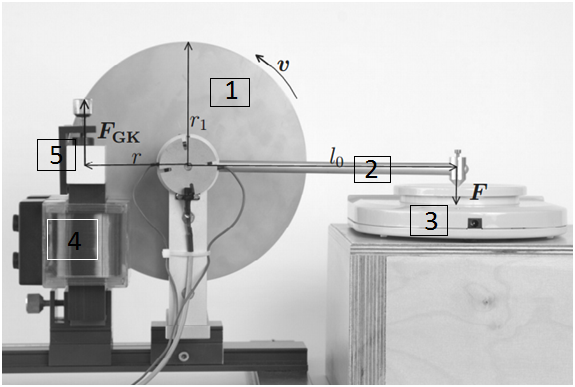
\includegraphics[scale=0.7]{Graphik/Versuchsaufbau}
\caption{Versuchsaufbau$^{\cite{A}}$}
\end{figure}

\begin{itemize}
\item[$\bullet$] 3 Metallscheiben (Aluminium, Messing, Edelstahl)
\item[$\bullet$] 	Spule
\item[$\bullet$] 	Elektromotor
\item[$\bullet$] 	Waage	
\item[$\bullet$] Strom und Spannungsmessgerät
\item[$\bullet$] Motorsteuergerät 
\item[$\bullet$] Stromquelle
\end{itemize}

\subsection{Versuchsaufbau}
Eine Metallscheibe (Kästchen 1) wird von dem Elektromotor angetrieben, dahinter ist ein Ausleger (Kästchen 2), der die Auflagekraft über die Waage (Kästchen 3) anzeigt. Um die Scheibe nun Abbremsen zu können, wird eine Spule (Kästchen 4) mit Polschuhen (Kästchen 5) dazwischen gestellt. Diese Spule erzeugt dann ein homogenes magnetisches Feld senkrecht zur Scheibe, die damit die Scheibe abbremst. Diesen Aufbau nennt man Wirbelstrombremse. 
~\\
\subsection{Versuchsdurchführung}

\subsubsection{Grundbelastung durch den Ausleger}
Als erstes wurde die Grundbelastung gemessen, diese entsteht aus dem Gewicht des Auslegers. Zusätzlich wurde noch die Belastung ohne Bremswirkung der Spule bei 1000\,$\frac{\text{U}}{\text{min}}$ gemessen

\subsubsection{Bremskraft in Abhängigkeit vom Radius}
In diesem Versuch wurden spitze Polschuhe verwendet, und die Drehzahl der Scheibe betrug 1000\,$\frac{\text{U}}{\text{min}}$. Der Spulenstrom betrug 400\,mA. 
Es wurde nur der Abstand der Spulen zur Achse der Scheibe von 50 - 100\,mm in 5\,mm Schritten verändert.
\subsubsection{Bremskraft in Abhängigkeit von der Drehzahl}
Im zweiten Versuch  war der Spulenstrom konstant mit 200 mA, gemessen wurde dann die Belastung durch die Drehzahl verändert, Drehzahl war von 250\,$\frac{\text{U}}{\text{min}}$ bis 2000\,$\frac{\text{U}}{\text{min}}$ in 250\,$\frac{\text{U}}{\text{min}}$ Schritten zu messen. Um später auch Vergleichswerte zu erhalten, wurde diese Messreihe einmal mit und einmal ohne Spulenstrom gemessen 

\subsubsection{Bremskraft in Abhängigkeit von der Magnetfeldstärke}
Die Drehzahl wird auf 1000\,$\frac{\text{U}}{\text{min}}$ eingestellt und der Spulenstrom wird von $50$\,mA auf den höchstmöglichen Spulenstrom in $50$\,mA Schritten erhöht.

\subsubsection{Bremskraft in Abhängigkeit von der Feldgeometrie}
Im nächsten Versuch wurden die breiten Polschuhe montiert und die ersten drei Versuche wiederholt.

\subsubsection{Bremskraft in Abhängigkeit von dem Scheibenmaterial}
In diesen Versuch wurden drei verschieden Scheiben getestet, Aluminium, Messing und Edelstahl. Die Spule hatte eine Stromstärke von 200\,mA und die Drehzahl betrug 1000\,$\frac{\text{U}}{\text{min}}$. Man betrachtete die maximale Bremskraft der Scheiben und verglich sie anschließend.

\subsubsection{Energiebetrachtung}
Die Drehzahl betrug 1000\,$\frac{\text{U}}{\text{min}}$ und das Strommessgerät wurde in den Motorstromkreis angeschlossen. Somit kann man die elektrische Antriebsleistung und den Wirkungsgrad ermitteln.

\subsubsection{Motor als Stromgenerator}
Diesmal wurde die Scheibe auf 2000\,$\frac{\text{U}}{\text{min}}$ beschleunigt und anschließend auf 250\,$\frac{\text{U}}{\text{min}}$ mit den Spulen, also im Generatorbetrieb, abgebremst, hierbei wurde die Zeit gestoppt. Um die Zahlen später vergleichen zu können wurde auch die Zeit gemessen, wie lange die Scheibe zum ausdrehen ohne Spule benötigt.

\newpage
\section{ Formeln}

\subsection{Formeln für Bremskraft und Bremsdrehmoment}
 \begin{equation}
 F=m_0\cdot g		
 \end{equation}
Wobei hier $F$ die Bremskraft in [N], $m_0$ die Grundbelastung der Waage und $g$ die Gravitationskonstante ist. \\
Daraus ergibt sich dann bei zusätzlicher Belastung der Waage eine Bremskraft:
\begin{equation}
F=(m-m_0) \cdot g     
\end{equation}
und damit als Bremsdrehmoment
\begin{equation}
M=l_0  \cdot F_g 
\end{equation}
Hier ist $M$ die Bremsdrehmoment in [Nm]	und $l_0 = 0,222$\,m die Auslegerlänge.\\
~\\
Für die Diskussionen in der Auswertung benötigen wir zudem für die Bremskraft, laut Versuchsanleitung (E45-14) folgende Formel:
\begin{equation}
F=\frac{b^2\cdot B^2 \cdot v}{R}=\frac{b^2\cdot B^2 \cdot  2\pi\cdot \frac{D}{60} \cdot r }{R}
\end{equation}
wozu wir $v=\omega \cdot r = 2\pi\cdot f \cdot r$ und $f=\frac{D}{60}$ für $D$ als Drehzahl, einsetzen.
Des weiteren ist \textbf{\textit{B}} das von der Spule erzeugte Magnetfeld in [T], R der elektrische Wirkwiderstand in [$\Omega$] und b die Breite des Feldes.
Daraus ergibt sich für das Drehmoment:
\begin{equation}
M=\frac{b^2\cdot B^2 \cdot v \cdot r}{R}=\frac{b^2\cdot B^2 \cdot  2\pi\cdot \frac{D}{60} \cdot r^2 }{R}
\end{equation}

%M_b=(b^2∙B^2∙〖ωr〗^2)/R		b= breite des Feldes					(4)
%													B= magnetische Feldstärke [T]
%                                          			R= elektrischer Widerstand [Ω] 
%			    	 								r= Radius 
%(M (breit))/M(spitz) 		M(breit)= Bremsdrehmoment mit breiten Polschuhen 	(5)
%									M(spitz) = Bremsdrehmoment mit spitzen Polschuhen 
\subsection{Formeln für die Leistung}
Für die mechanische Bremsleistung ergeben sich folgende Formeln:
\begin{equation}
P_{mech}=F \cdot v	
\end{equation}
Wobei $P_{mech}$  die mechanische Bremsleistung in [W]	ist und $v$ die Geschwindigkeit	.
Für die elektrische Bremsleistung gilt:
\begin{equation}
P_{el}=U \cdot I
\end{equation} 
Mit $U$ als Spannung und $I$ als Strom.
Durch einsetzen von $v=\omega \cdot r = 2\pi\cdot f \cdot r$ und $f=\frac{D}{60}$ für $D$ als Drehzahl.
\begin{equation}
P_{mech}=(m-m_0) \cdot g\cdot l_0 \cdot 2\pi\cdot \frac{D}{60}		
\end{equation}

\newpage
\section{ Messwerte}
\begin{figure}[h]
\vspace{-20pt}
\centering
\caption{Messwerte in Abhängigkeit vom Radius}
\begin{tabular}{|c|c|c|c|c|}\hline 
Radius $r$ [mm] & Masse $m$ [g]  \\ \hline 
50		&47,40 \\ \hline 
55		&48,90 \\ \hline 
60		&50,50 \\ \hline 
65		&53,20 \\ \hline 
70		&54,50 \\ \hline 
75		&56,30 \\ \hline 
80		&57,90 \\ \hline 
85		&59,01 \\ \hline 
90		&58,00 \\ \hline 
95		&52,50 \\ \hline 
100		&41,90 \\ \hline 
\end{tabular} \\
\end{figure}

\begin{figure}[h]
\vspace{-20pt}
\centering
\caption{Messwertein Abhängigkeit von der Drehzahl}
\begin{tabular}{|c|c|c|}\hline 
& Mit Spulenstrom & ohne Spulenstrom \\ \hline 
Drehzahl [$\frac{\text{U}}{\text{min}}$] &Masse $m$ [g]  &Masse $m$ [g] \\ \hline 
250&	33,00&	32,00\\ \hline 
500&	35,10&	32,10\\ \hline 
750&	37,10&	32,60\\ \hline 
1000&	39,10&	32,70\\ \hline 
1250&	40,20&	33,10\\ \hline 
1500&	41,40&	33,40\\ \hline 
1750&	43,00&	33,80\\ \hline 
2000&	44,30&	34,30\\ \hline 
\end{tabular} \\
\end{figure} 
\begin{figure}[h]
\vspace{-20pt}
\centering
\caption{Messwerte für den Motor}
\begin{tabular}{|c|c|}\hline 
Auf Spule umgeschaltet & Drehzahl runter gedreht\\ \hline 
Zeit $t$ [s] & Zeit $t$ [s] 	\\ \hline 
7,43 & 101,47		\\ \hline 
7,46	& 99,63		\\ \hline 
7,49 & 99,70	\\ \hline 
\end{tabular} \\
\end{figure}
\noindent
\begin{figure}[h]
\vspace{-20pt}
\centering
\caption{Messwerte in Abhängigkeit von der Magnetfeldstärke}
\begin{tabular}{|c|c|}\hline 
Spulenstrom I [mA] & Masse $m$ [g]  \\ \hline 
50	&33,45\\ \hline 
100	&34,50\\ \hline 
150	&36,20\\ \hline 
200	&38,50\\ \hline 
250	&41,60\\ \hline 
300	&45,30\\ \hline 
350	&49,70\\ \hline 
400	&53,30\\ \hline 
450	&61,00\\ \hline 
500	&67,60\\ \hline 
550	&74,60\\ \hline 
600	&83,20\\ \hline 
\end{tabular} \\
\end{figure}
\begin{figure}[h]
\vspace{-20pt}
\centering
\caption{Messwerte in Abhängigkeit von der Feldgeometrie}
\begin{tabular}{|c|c|}\hline 
Drehzahl [$\frac{\text{U}}{\text{min}}$] &Masse $m$ [g]\\ \hline 
250	&38,60\\ \hline 
500	&44,70\\ \hline 
750	&50,20\\ \hline 
1000	&57,00\\ \hline 
1250	&60,90\\ \hline 
1500	&65,40\\ \hline 
1750	&69,20\\ \hline 
\end{tabular} 
\begin{tabular}{|c|c|}\hline 
Spulenstrom I [mA] & Masse $m$ [g] \\ \hline 
50	&35,70\\ \hline 
100	&41,40\\ \hline 
150	&50,20\\ \hline 
200	&57,20\\ \hline 
250	&71,00\\ \hline 
\end{tabular} \\
\end{figure}
\begin{figure}[h]
\vspace{-20pt}
\centering
\caption{Messwerte in Abhängigkeit vom Scheibenmaterial}
\begin{tabular}{|c|c|c|c|}\hline 
Material &	Spulenstrom I [mA]	& Masse $m$ [g]	& Grundbelastung $m_0$ [g]\\ \hline 
Alu	&200	&68,90	&32,80\\ \hline 
Messing	&200	&59,10	&31,80\\ \hline 
Edelstahl	&200	&35,60	&32,80\\ \hline 
\end{tabular} \\
\end{figure}
\begin{figure}[h]
\vspace{-20pt}
\centering
\caption{Messwerte für die Energiebetrachtung}
\begin{tabular}{|c|c|c|c|}\hline 
Spulenstrom I [mA]	& Spannung in [V] & gemessener Strom   [A] & Masse $m$ [g]	\\ \hline 
100	&6	&0,35	&40,30	\\ \hline 
200	&8	&1,10	&58,70	\\ \hline 
\end{tabular} \\
\end{figure}
\noindent

\newpage
\clearpage
\section{ Auswertung}

\subsection{Grundbelastung durch den Ausleger}
Im ersten Teil des Versuchs wurde eine Grundbelastung von $31,80$\,g gemessen und bei $1000\,\frac{\text{U}}{\text{min}}$ erhalten wir eine Grundbelastung von $m=33,1$\,g.
Dieser wird bei allen Versuchen, in denen  $1000\,\frac{\text{U}}{\text{min}}$ verwendet wurde abgezogen. 

\subsection{Bremskraft in Abhängigkeit vom Radius}
Für die Berechnung der Bremskraft und des Bremsdrehmomentes wird hier ein Beispiel mit Radius $r=50$\,mm und dem dementsprechenden gemessenen Gewicht $47,4$\,g.
Dazu benutzen wir Formel (2) und (3):
\begin{align*}
F&=(m-m_0) \cdot g = (47,4\cdot 10^{-3}\,\text{kg}-33,1\cdot 10^{-3}\,\text{kg})\cdot 9,81\,\frac{\text{m}}{\text{s}^2}=0,1428\,\text{N}=140,30\,\text{mN}  \\
~\\
M&=l_0  \cdot F_g = 0,1428\,\text{N} \cdot 0,222\,\text{m} = 0,03114\,\text{Nm}=31,14\,\text{mNm}
\end{align*}
Im Anschluss werden alle weiteren errechneten Werte in einer Tabelle dargestellt, wobei hier die Masse gleich ohne Grundbelastung angegeben wird:
\begin{figure}[h]
\centering
\caption{Ergebnisse Bremskraft und Bremsdrehmoment}
\begin{tabular}{|c|c|c|c|c|}\hline 
Radius $r$ [mm] & Masse $m$ [g] & Bremskraft $F$ [mN] & Bremsdrehmoment $M$ [mNm] \\ \hline 
50	&16,9	&140,28	&31,14 \\ \hline 
55	&21,9	&155,00	&34,41 \\ \hline 
60	&26,9	&170,69	&37,89 \\ \hline 
65	&31,9	&197,18	&43,77 \\ \hline 
70	&36,9	&209,93	&46,61 \\ \hline 
75	&41,9	&227,59	&50,53 \\ \hline 
80	&46,9	&243,29	&54,01 \\ \hline 
85	&51,9	&255,06	&56,62 \\ \hline 
90	&56,9	&244,27	&54,23 \\ \hline 
95	&61,9	&190,31	&42,25 \\ \hline 
100	&66,9	&86,33	&19,16 \\ \hline 
\end{tabular} \\
\end{figure} \\
~\\
Zu guter Letzt wird ein Diagramm, dass die Abhängigkeit von Bremsdrehmoment zum Radius darstellt: \\
\begin{figure}[h]
\centering
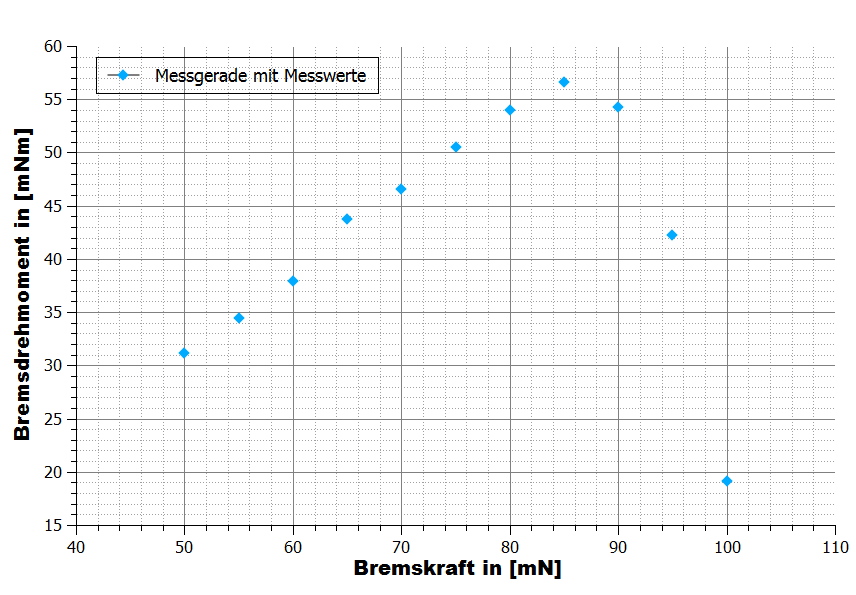
\includegraphics[scale=0.7]{Graphik/Radius}
\caption{Bremsdrehmoment in Abhängigkeit vom Radius}
\end{figure}
\newpage
\noindent
Bis zum Radius $r=85$\,mm steigt das Bremsdrehmoment linear, nach diesem Punkt nimmt das Bremsdrehmoment stark ab. Dies ist dadurch zu erklären, dass nach diesem Punkt das Magnetfeld kaum noch Einfluss auf das Scheibenmaterial hat, bzw. bei $r=100$\,mm gar nicht. \\
\newpage
\subsection{Bremskraft in Abhängigkeit von der Drehzahl}
Die Bremskraft und das Bremsdrehmoment wird hier an einem Beispiel der Drehzahl $250\,\frac{\text{U}}{\text{min}}$ und dem dementsprechenden 
gemessenen Gewicht $33,0$\,g bei aktivierten Spulenstrom und $32,0$\,g ohne Spulenstrom. Hier ist $F_{Sp}$ die Bremskraft bei aktivierten Spulenstrom 
und $F$ ohne Spulenstrom. Dazu benutzen wir wieder Formel (2) und (3):
\begin{align*}
F_{Sp}&=(m-m_0) \cdot g = (33,0\cdot 10^{-3}\,\text{kg}-31,8\cdot 10^{-3}\,\text{kg})\cdot 9,81\,\frac{\text{m}}{\text{s}^2}=0,01177\,\text{N}=11,77\,\text{mN}  \\
~\\
M_{Sp}&=l_0  \cdot F_{Sp} = 0,01177\,\text{N} \cdot 0,222\,\text{m} = 0,00261\,\text{Nm}=2,61\,\text{mNm}\\
~\\
F&=(m-m_0) \cdot g = (32,0\cdot 10^{-3}\,\text{kg}-31,8\cdot 10^{-3}\,\text{kg})\cdot 9,81\,\frac{\text{m}}{\text{s}^2}=0,00196\,\text{N}=1,96\,\text{mN}  \\
~\\
M&=l_0  \cdot F = 0,01177\,\text{N} \cdot 0,222\,\text{m} = 0,00044\,\text{Nm}=0,44\,\text{mNm}
\end{align*}
In folgender Tabelle werden die restlichen Werte dargestellt:
\begin{figure}[h]
\centering
\caption{Ergebnisse Bremskraft und Bremsdrehmoment}
\begin{tabular}{|c|c|c|c|c|c|}\hline 
Drehzahl [$\frac{\text{U}}{\text{min}}$] & Bremskraft $F_{Sp}$ [mN] & Drehmoment $M_{Sp}$ [mNm] &  $F$ [mN] &  $M$ [mNm] \\ \hline 
250		&11,77		&1,96		&2,61		&0,44\\ \hline 
500		&32,37	&2,94		&7,19		&0,65\\ \hline 
750		&51,99	&7,85		&11,54		&1,74\\ \hline 
1000	&71,61	&8,83		&15,90	&1,96\\ \hline 
1250	&82,40	&12,75	&18,29	&2,83\\ \hline 
1500	&94,18	&15,70	&20,91	&3,48\\ \hline 
1750	&109,87	&19,62	&24,39	&4,36\\ \hline 
2000	&122,63	&24,53	&27,22	&5,44\\ \hline 
\end{tabular} \\
\end{figure} \\
Auch hier wird ein Diagramm erstellt, dass die Abhängigkeit von Bremsdrehmoment zur Drehzahl darstellt:
\begin{figure}[h]
\centering
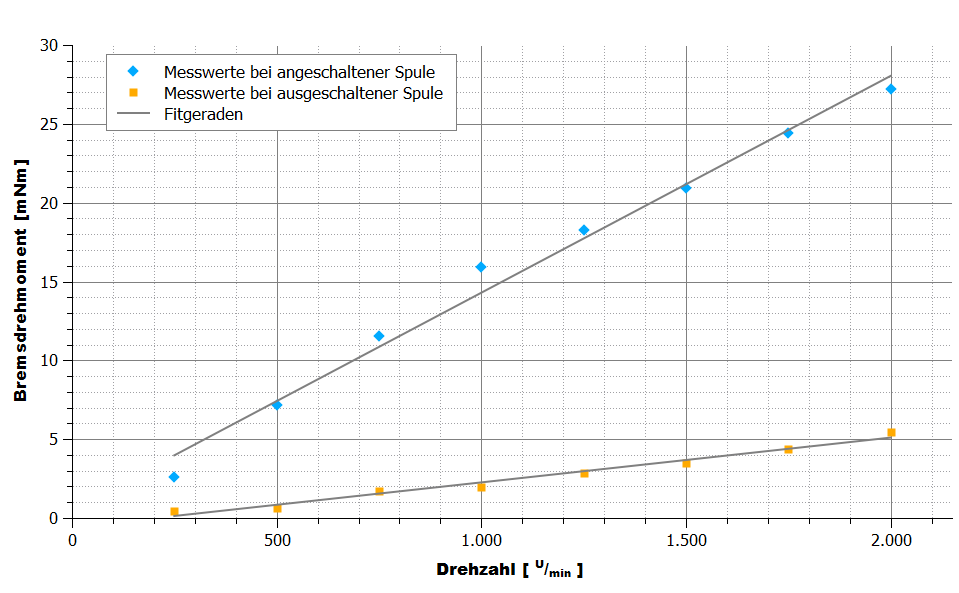
\includegraphics[scale=0.65]{Graphik/Drehzahl}
\caption{Bremsdrehmoment in Abhängigkeit zur Umdrehung}
\end{figure}\\
\newpage
\noindent
Mit Hilfe von Formel (5)  erhalten wir hier, in der Theorie, eine Proportionalität von Bremsdrehmoment (und auch die Bremskraft) zur Drehzahl $D$. Aus unseren Werten und unserem Diagramm erhalten wir ebenfalls die Proportionalität, die in unserem Diagramm nochmal durch Fitgeraden $a_i x + b_i$ verdeutlicht wird.
Ebenfalls wird anschaulich, dass durch Ausschalten der Spule das Magnetfeld kleiner wird und dadurch auch das Bremsdrehmoment.

\subsection{Bremskraft in Abhängigkeit von der Magnetfeldstärke}
Auch hier wird eine Beispielrechnung vollführt und zwar für den Radius $r=50$\,mm und dem dementsprechend gemessenen Gewicht $47,4$\,g.
Wir benötigen:
\begin{align*}
F&=(m-m_0) \cdot g = (33,45\cdot 10^{-3}\,\text{kg}-33,1\cdot 10^{-3}\,\text{kg})\cdot 9,81\,\frac{\text{m}}{\text{s}^2}=0,01619\,\text{N}=16,19\,\text{mN}  \\
~\\
M&=l_0  \cdot F_g = 0,01619\,\text{N} \cdot 0,222\,\text{m} = 0,00359\,\text{Nm}=3,59\,\text{mNm}
\end{align*}
In der nachfolgenden Tabelle sind alle errechneten Werte aufgeführt:
\begin{figure}[h]
\centering
\caption{Ergebnisse Bremskraft und Bremsdrehmoment}
\begin{tabular}{|c|c|c|}\hline 
Spulenstrom I [mA] & Bremskraft $F$ [mN] & Drehmoment $M$ [mNm] \\ \hline 
50	&16,19		&3,59\\ \hline 
100	&26,49		&5,88\\ \hline 
150	&43,16		&9,58\\ \hline 
200	&65,73		&14,59\\ \hline 
250	&96,14		&21,34\\ \hline 
300	&132,44		&29,40\\ \hline 
350	&175,60		&38,98\\ \hline 
400	&210,92		&46,82\\ \hline 
450	&286,45		&63,59\\ \hline 
500	&351,20		&77,97\\ \hline 
550	&419,87		&93,21\\ \hline 
600	&504,23		&111,94\\ \hline 
\end{tabular} \\
\end{figure}
\newpage
\noindent
Damit erhalten wir folgendes Diagramm:
\begin{figure}[h!]
\centering
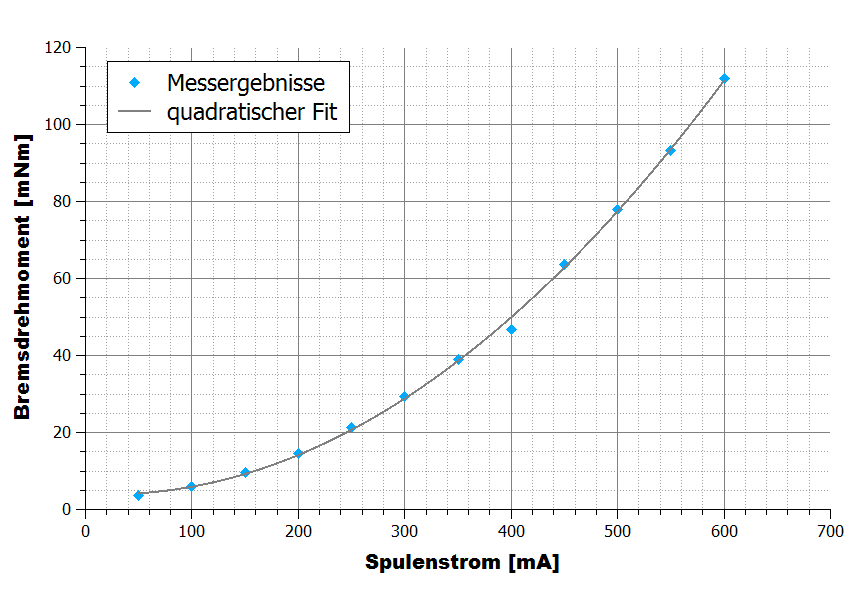
\includegraphics[scale=0.65]{Graphik/Spule}
\caption{Bremsdrehmoment in Abhängigkeit zum Spulenstrom}
\end{figure}\\
Auch  hier wird mit Hilfe der Formel (5) der quadratische Anstieg klar, da steigende, Spulenstrom auch die Magnetfeldstärke  \textbf{\textit{B}} steigt. Mit der Fitkurve $ax^2 +bx+ c$ wird der quadratische Anstieg nochmals verdeutlicht.

\subsection{Bremskraft in Abhängigkeit von der Feldgeometrie}
Verwenden wird die breiten Polschuhe und führen die Versuchsteile 6.1-6.4 nochmals durch, ergebt sich folgendes:\\

\subsubsection{Abhängigkeit Radius}
Die Bremskraft ist so stark, dass wir lediglich für den Radius $r=95$\,mm und $r=100$\,mm angemessene Messwerte erhalten. 
Schauen wir uns Formel (5) an, so sehen wir das das Bremsdrehmoment proportional zum Quadrat der Breite der Polschuhe ist. Die Durchmesser der breiten Polschuhe ist dreimal höher als die spitzen Polschuhe und man erhält daher, dass sich das Bremsdrehmoment verneunfacht. Doch verhält sich der Wirkwiderstand, laut Versuchsanleitung, $R$ proportional zur Breite $b$, d.h. bei breiten Polschuhen wird  der Widerstand verdreifacht.  Für unsere Formel ergibt sich also zusammenfassend eine Verdreifachung der Bremsdrehmoments.  Analog wird auch die Bremskraft verdreifacht und daher ist die Bremskraft bis zum Radius $r=95$\,mm so stark, dass sich nichts tut. 

\subsubsection{Abhängigkeit Drehzahl}
Da die Drehzahl nicht von der Breite der Polschuhe nicht abhängt, wird auch hier das Bremsdrehmoment für breite Polschuhe verdreifacht. Wie wir schon in 6.3 herausgefunden haben, verhält sich das Bremsdrehmoment linear zur Drehzahl. Deswegen ist bei kleinen Umdrehungen es für uns möglich gewesen, eine Bremskraft bzw. eine Bremsdrehmoment zu errechnen.

\subsubsection{Abhängigkeit Spulenstrom}
Da auch der Spulenstrom in keiner unmittelbaren Abhängigkeit zur Breite der Polschuhe steht, wird hier das Drehmoment auch um das dreifache größer sein. Die quadratische Abhängigkeit Spulenstrom und Bremsdrehmoment erlaubt es uns, für kleine Ströme eine Bremskraft und damit eine Bremsdrehmoment zu errechnen.

\subsubsection{Ergebnisse für breite Polschuhe}	
Die folgenden Tabellen enthalten alle errechneten Bremsdrehmomente für die breiten Polschuhe:
\begin{figure}[h!]
\begin{minipage}{1\textwidth}
\centering
\caption{Ergebnisse Bremskraft und Bremsdrehmoment}
\begin{tabular}{|c|c|c|c|c|c|}\hline 
Drehzahl [$\frac{\text{U}}{\text{min}}$] & Bremskraft $F_{Sp}$ [mN] & Drehmoment $M_{Sp}$ [mNm]  \\ \hline 
250		&66,71		&14,81\\ \hline 
500		&126,55		&28,09\\ \hline 
750		&180,50		&40,07\\ \hline 
1000	&247,21		&54,88\\ \hline 
1250	&285,47		&63,37\\ \hline 
1500	&329,62		&73,17\\ \hline 
\end{tabular} \\
\end{minipage}
\begin{minipage}{1\textwidth}
\centering
\caption{Ergebnisse Bremskraft und Bremsdrehmoment}
\begin{tabular}{|c|c|c|}\hline 
Spulenstrom I [mA] & Bremskraft $F$ [mN] & Drehmoment $M$ [mNm] \\ \hline 
50	&38,26		&8,49\\ \hline 
100	&94,18		&20,91\\ \hline 
150	&180,50	&40,07\\ \hline 
200	&249,17	&55,32\\ \hline 
250	&384,55	&85,37\\ \hline 
\end{tabular} \\
\end{minipage}
\end{figure}
Vergleicht man die Drehmomente für breite und spitze Polschuhe, so ergibt sich immer ein Verhältnis von etwas mehr als  4. Dieses höhere Verhältnis lässt sich durch Messungenauigkeiten, auf die in den Fehlerquellen eingegangen wird, erklären.
\newpage

\subsection{Bremskraft in Abhängigkeit von dem Scheibenmaterial}
Durch  ermitteln der größtmöglichen Bremskraft für Aluminium, welches bei  $1000\,\frac{\text{U}}{\text{min}}$ für $200$\,mA lag, können wir die Abhängigkeit des Scheibenmaterials überprüfen. Dazu gibt es wieder eine Beispielrechnung für Aluminium für die Grundmasse von $m=36,1$\,g:
\begin{align*}
F&=(m-m_0) \cdot g = (36,1\cdot 10^{-3}\,\text{kg})\cdot 9,81\,\frac{\text{m}}{\text{s}^2}=0,3541\,\text{N}=354,14\,\text{mN}  \\
~\\
M&=l_0  \cdot F_g = 0,3541\,\text{N} \cdot 0,222\,\text{m} = 0,07862\,\text{Nm}=78,62\,\text{mNm}
\end{align*}
Die anderen Ergebnisse sind in der Tabelle eingetragen: 
\begin{figure}[h]
\centering
\caption{Ergebnisse Bremskraft und Bremsdrehmoment}
\begin{tabular}{|c|c|c|c|}\hline 
Material	&Grundmasse $m$ & 		Bremskraft $F$ [mN] & Drehmoment $M$ [mNm] \\ \hline 
Alu			&36,10		&354,14		&78,62 \\ \hline 
Messing	&7,30		&267,81		&59,45 \\ \hline 
Edelstahl	&2,80		&27,47		&6,10 \\ \hline 
\end{tabular} \\
\end{figure} \\
Im Anschluss werden alle Verhältnisse miteinander berechnet und gleich mit dem Literaturwert verglichen: \\
\begin{figure}[h]
\centering
 \setlength{\tabcolsep}{20mm}
\begin{tabular}{c|c}
gemessen & Literatur$^{\cite{2}}$\\
~\\
$\frac{M_{Alu}}{M_{Messing}} = \frac{78,62\,\text{mNm}}{59,45\,\text{mNm}} = 1,32$ & $\frac{\sigma_{Alu}}{\sigma_{Messing}}= \frac{36,59 \cdot 10^6\,\frac{1}{\Omega\cdot \text{m}}}{15,5 \cdot 10^6\,\frac{1}{\Omega\cdot \text{m}}}= 2,36$\\
~\\
$\frac{M_{Alu}}{M_{Edelstahl}} = \frac{78,62\,\text{mNm}}{6,10\,\text{mNm}} = 12,89$ & $\frac{\sigma_{Alu}}{\sigma_{Edelstahl}}= \frac{36,59 \cdot 10^6\,\frac{1}{\Omega\cdot \text{m}}}{1,4 \cdot 10^6\,\frac{1}{\Omega\cdot \text{m}}}= 26,14$\\
~\\
$\frac{M_{Messing}}{M_{Edelstahl}} = \frac{59,45\,\text{mNm}}{6,10\,\text{mNm}} = 9,75$ & $\frac{\sigma_{Messing}}{\sigma_{Edelstahl}}= \frac{15,5 \cdot 10^6\,\frac{1}{\Omega\cdot \text{m}}}{1,4 \cdot 10^6\,\frac{1}{\Omega\cdot \text{m}}}= 11,07$\\
\end{tabular} 
\end{figure}\\
\newpage
\noindent
Der Vergleich mit den Literaturwerten ergibt, dass wir bei jedem Verhältnis drunter liegen.

\subsection{Energiebetrachtung}

\subsubsection{Berechnung der Leistungen}

Für die Energiebetrachtung benötigen wir erst $P_{\text{mech}}$ und $P_{\text{el}}$ für einen Spulenstrom von jeweils $100$\,mA und $200$\,mA. 
Dazu benötigen wir Formel (7) und (8):
\begin{align*}
P_{\text{el}_{100\,\text{mA}}}&=U \cdot I = 6\,\text{V}\cdot 0,35\,\text{A}=2,1\,\text{W} \\
P_{\text{el}_{200\,\text{mA}}}&=U \cdot I = 8\,\text{V}\cdot1,1\,\text{A}=8,8\,\text{W} \\
~\\
P_{\text{mech}_{100\,\text{mA}}}&=(m-m_0) \cdot g\cdot l_0 \cdot 2\pi\cdot \frac{D}{60}	= (40,3-33,1)\cdot 10^{-3}\,\text{kg} \cdot 9,81\,\frac{\text{m}}{\text{s}^2} \cdot 0,07\,\text{m} \cdot 2\pi \cdot \frac{100}{60\,\text{s}}	\\
&= 0,52\,\text{W} \\
P_{\text{mech}_{100\,\text{mA}}}&=(m-m_0) \cdot g\cdot l_0 \cdot 2\pi\cdot \frac{D}{60} = (58,7-33,1)\cdot 10^{-3}\,\text{kg} \cdot 9,81\,\frac{\text{m}}{\text{s}^2} \cdot 0,07\,\text{m} \cdot 2\pi \cdot \frac{100}{60\,\text{s}}	\\
&= 1,84\,\text{W}		
\end{align*}

\subsubsection{Wirkungsgrade}
Ein Ziel des Versuchs ist es, den Wirkungsgrad des Motors zu bestimmen. Dafür benötigen wir $P_{\text{mech}}$ und $P_{\text{el}}$, die wir gerade berechnet haben. Wir erhalten folgende Wirkungsgrade:
\begin{align*}
\eta_{\text{100\,\text{mA}}}=\frac{P_{\text{mech}_{100\,\text{mA}}}}{P_{\text{el}_{100\,\text{mA}}}} = \frac{0,52\,\text{W}}{2,1\,\text{W}}=0,25\\
\eta_{\text{200\,\text{mA}}}=\frac{P_{\text{mech}_{200\,\text{mA}}}}{P_{\text{el}_{200\,\text{mA}}}} = \frac{1,84\,\text{W}}{8,8\,\text{W}}=0,21
\end{align*}
Die Wirkungsgrade sind zumindest realistisch und liegen nah aneinander. Weitere Aussagen können wir erst nach der Fehlerrechnung machen.
\newpage
\subsection{Motor als Stromgenerator}

\subsubsection{Motor mit aktiver Spule}
Nach einer Beschleunigung auf $2000\,\frac{\text{U}}{\text{min}}$ wird auf Generatorbetrieb geschaltet. Wie aus den Messwerten ersichtlich, ist der Motor nach etwa $7,46$\,s auf  
$500\,\frac{\text{U}}{\text{min}}$ runtergefahren. Die Rotationsenergie \glqq verschwindet\grqq in Form von Wärme- und Reibungsenergie.

\subsubsection{Motor ohne aktive Spule}
Wieder wird nach einer Beschleunigung auf $2000\,\frac{\text{U}}{\text{min}}$ auf  auf Generatorbetrieb geschaltet. Aus den Messwerten ergibt sich, dass erst nach etwa 100\,s auf 
$500\,\frac{\text{U}}{\text{min}}$ runtergefahren. Auch hier \glqq verschwindet\grqq die Rotationsenergie  in Form von Wärme- und Reibungsenergie, allerdings ist die Reibungsenergie hier geringer.

\section{Fehlerquellen und Fehlerrechnung}

\subsection{Fehlerquellen}
Die größte Fehlerquelle in diesem Versuch war die Waage. Die Waage variierte sehr oft das Gewicht und das führte dazu, dass bei jeder Messung ein unserer Meinung angemessener Wert 
genommen wurde. Angemessen heißt in diesem Fall, dass wir etwas warteten und dann ungefähr den Mittelwert aus dem höchsten erreichten und niedrigsten erreichten Wert nahmen. Ebenfalls 
eine relativ große Fehlerquelle ist die menschliche Reaktionszeit. Bei der Zeitmessung hatten wir im ersten Teil nur sieben Sekunden, mit einer Reaktionszeit von einer Sekunde ist der Fehler nicht 
zu verachten. Natürlich haben alle Messapparaturen ihre Toleranzen. Für diesen Versuch nehmen wir also folgende Fehler an:\\
~\\
\begin{figure}[h]
\vspace{-25pt}
\centering
\begin{tabular}{ll}
Fehlerquelle 	& Messungenauigkeit \\ \hline
~\\
Masse			&	$\pm 0,1\,$g \\
Zeit				& $\pm 1\,$s \\
Drehzahl		& $\pm 5\,\frac{\text{Umdrehung}}{\text{min}}$ \\
Stromstärke 	& $\pm 10$\,mA\\
Spannung: 	& $\pm0,1$\,V \\
\end{tabular} \\
\end{figure}\\

\newpage

\subsection{Fehlerrechnung}
Wir diesen Versuch sollen wir noch eine Fehlerrechnung für den Wirkungsgrad $\eta$ machen.\\
Die Formel für den Wirkungsgrad ist:
\begin{align*}
\eta =\frac{P_{\text{mech}}}{P_{\text{el}}}= \frac{m \cdot g \cdot l_0 \cdot 2\pi \cdot \frac{D}{60}}{U\cdot I}
\end{align*}
Mit etwas Vorüberlegung können wir uns ein $h$ so definieren, dass:
\begin{align*}
h \define\frac{g \cdot l_0 \cdot 2\pi }{60\,\text{s}} = \frac{9,81\,\text{m} \cdot 0,222\,\text{m}  \cdot 2\pi}{60\cdot\text{s}^3} = 0,23\,\frac{\text{m}^2 }{\text{s}^3}
\end{align*}
$h$ hat die Einheit $[\frac{2\pi\cdot\text{m}^2 }{60\cdot \text{s}^3}]$. \\
Das macht unsere Fehlerrechnung etwas kürzer und übersichtlicher. Es gilt nun für $\Delta\eta$:\\
\begin{align*}
\Delta\eta_{\text{100\,mA}} &	= \l \frac{h \cdot D}{U\cdot I} \r \cdot \Delta m 
			+ \l \frac{h \cdot m}{U\cdot I} \r \cdot \Delta D 
			+ \l \frac{h \cdot D \cdot m}{U^2\cdot I} \r \cdot \Delta U
			+ \l \frac{h \cdot D \cdot m}{U\cdot I^2} \r \cdot \Delta I & \\
			& = \l \frac{0,23\,\frac{\text{m}^2 }{\text{s}^3} \cdot 1000}{6\,\text{V}\cdot 0,35\,\text{A}} \r \cdot 0,1\cdot 10^{-3}\,\text{kg}
			+ \l \frac{0,23\,\frac{\text{m}^2 }{\text{s}^3} \cdot (40,3-33,1)\cdot 10^{-3}\,\text{kg}}{6\,\text{V}\cdot 0,35\,\text{A}} \r \cdot 5 &\\
			& + \l \frac{0,23\,\frac{\text{m}^2 }{\text{s}^3} \cdot (40,3-33,1)\cdot 10^{-3}\,\text{kg} \cdot 1000}{(6\,\text{V})^2\cdot 0,35\,\text{A}} \r \cdot  0,1\,\text{V}&\\
			& + \l \frac{0,23\,\frac{\text{m}^2 }{\text{s}^3} \cdot (40,3-33,1)\cdot 10^{-3}\,\text{kg} \cdot 1000}{6\,\text{V}\cdot (0,35\,\text{A})^2} \r \cdot  10\cdot 10^{-3}\,\text{A}&\\
			& = 0,05 &\\
\end{align*}
und für $\Delta\eta_{\text{200\,mA}}$ ergibt sich:\\
\begin{align*}
\Delta\eta_{\text{200\,mA}} &= 0,02
\end{align*}


\newpage

\section{Zusammenfassung}
Ziel des Versuchs war es die verschiedensten Abhängigkeiten für die Bremskraft, bzw. den Bremsdrehmoment, einer Wirbelstrombremse auszuwerten.
Zudem wurde die Funktionsweise als Motor betrachtet und der Wirkungsgrad der Wirbelstrombremse errechnet.\\
~\\
Zuallererst schauten wir uns die Abhängigkeit vom Bremsdrehmoment zum Radius. Wir erhielten eine linearen anstieg bis zum Radius $r= 85\,$mm. Danach fiel das Drehmoment stark ab. Dies ist dadurch zu erklären, dass das Magnetfeld kaum noch Einfluss auf das Scheibenmaterial ab einem bestimmten Radius hat.\\
~\\
Danach wurde die Abhängigkeit Bremsdrehmoment-Drehzahl untersucht. Wir erhielten einen linearen Anstieg, was mit der Theorie übereinstimmt, wie aus Formel (5) ersichtlich.\\
~\\
Nun war die Abhängigkeit Bremsdrehmoment-Magnetfeldstärke dran. Wir erhielten einen quadratischen Anstieg für steigendes \textbf{\textit{B}}. Auch hier bestätigt Formel (5), dass unsere Ergebnisse mit der Theorie übereinstimmen.
~\\
Im nächsten Versuchsteil wurden nun breitere Polschuhe verwendet und erhielten aus unseren theoretischen Überlegungen, dass sich für die breiteren Polschuhe das Bremsdrehmoment verdreifachen sollte. Aus unseren Ergebnissen erhielten wir einen Faktor zwischen 4 und 5. Eine Begründung wäre die Messungenauigkeiten, die der Versuch so mit sich bringt.\\
~\\
Bei der Abhängigkeit zum Scheibenmaterial sind wir immer unter den Literaturwerten geblieben. Interessanterweise ist das Verhältnis von Alu zu Messing und Alu zu Edelstahl um etwa den Faktor 2 kleiner. \\
~\\
Für die Energiebetrachtung berechneten wir erst $P_{\text{mech}}$ und $P_{\text{el}}$ und erhielten bei  $P_{\text{el}}$ bei einer Verdopplung des Spulenstroms eine Vervierfachung der Leistung. Bei $P_{\text{mech}}$ erhielten wir für den doppelten Spulenstrom eine Verdreifachung der Leistung.\\
Das spiegelt sich dann auch beim Wirkungsgrad, so ist der Wirkungsgrad für $200$\,mA Spulenstrom etwas kleiner. Jedoch ist der Fehler auch etwas kleiner. So erhalten wir insgesamt für den Wirkungsgrad:
\begin{align*}
\eta_{\text{100\,\text{mA}}} \pm \Delta \eta_{\text{100\,\text{mA}}}=0,25 \pm  0,05\\
\eta_{\text{200\,\text{mA}}} \pm \Delta \eta_{\text{200\,\text{mA}}}=0,21 \pm  0,02
\end{align*}\\
Im letzten Versuchsteil erhielten wir als Ergebnis, dass mit angeschalteter Spule, die Reibungsenergie deutlich höher ist und damit unweigerlich auch die Bremskraft. 
\newpage
         
\section{Literaturverzeichnis}
 \renewcommand\refname{~}
 \vspace{-25pt}

\begin{thebibliography}{xxx}
\bibitem{1}		\glqq \textit{E45 Wirbelstrombremse}\grqq, in\\
						\textit{http:www3.physik.uni-stuttgart.de/studium/praktika/ap/}, unter\\
						\textit{http://www3.physik.uni-stuttgart.de/studium/praktika/ap/pdf\_dateien/E45.pdf}; \\
						abgerufen am 04.06.2015
\bibitem{2}		\textit{http://de.wikipedia.org/wiki/Elektrische\_Leitfähigkeit} \\
						unter Kapitel \glqq \text{4 Elektrische Leitfähigkeit verschiedener Stoffe}\grqq \\
						abgerufen am 04.06.2015
\bibitem{A}		Graphik aus \glqq \textit{E45 Wirbelstrombremse}\grqq, in\\
						\textit{http://www3.physik.uni-stuttgart.de/studium/praktika/ap/}, unter \\
						\textit{http://www3.physik.uni-stuttgart.de/studium/praktika/ap/bilder/?Name=E45.jpg}; \\
						abgerufen am 04.06.2015
\end{thebibliography}

\section{Anhang}


\end{document}
